%%%%%%%%%%%%%%%%%%%%%%%%%%%%%%%%%%%%%%%%%%%%%%%%%%%%%%%%%%%%%%%%%%%%%%%
% Info
%%%%%%%%%%%%%%%%%%%%%%%%%%%%%%%%%%%%%%%%%%%%%%%%%%%%%%%%%%%%%%%%%%%%%%%
% Author: Louis Pahlavi
% Email:  louis.pahlavi@mail.utoronto.ca

% This is my personal resume. All the document setup is made inside the
% "Resume" template.

%%%%%%%%%%%%%%%%%%%%%%%%%%%%%%%%%%%%%%%%%%%%%%%%%%%%%%%%%%%%%%%%%%%%%%%
% General setup
%%%%%%%%%%%%%%%%%%%%%%%%%%%%%%%%%%%%%%%%%%%%%%%%%%%%%%%%%%%%%%%%%%%%%%%
\documentclass{ResumeTemplate}

%%%%%%%%%%%%%%%%%%%%%%%%%%%%%%%%%%%%%%%%%%%%%%%%%%%%%%%%%%%%%%%%%%%%%%%
% Document
%%%%%%%%%%%%%%%%%%%%%%%%%%%%%%%%%%%%%%%%%%%%%%%%%%%%%%%%%%%%%%%%%%%%%%%
\begin{document}

    \fontsize{12}{12}\selectfont

    %%%%%%%%%%%%%%%%%%%%%%%%%%%%%%%%%%%%%%%%%%%%%%%%%%%%%%%%%%%%%%%%%%%
    % Name
    %%%%%%%%%%%%%%%%%%%%%%%%%%%%%%%%%%%%%%%%%%%%%%%%%%%%%%%%%%%%%%%%%%%
    \centering\myname{Louis L. W. D. Pahlavi}
    \vspace{1cm}
    % \raggedright\begin{minipage}[c]{0.64\linewidth}
    % \end{minipage}
    % \hspace{0.01\linewidth}
    % \raggedright\begin{minipage}[c]{0.33\linewidth} 
    %     \centering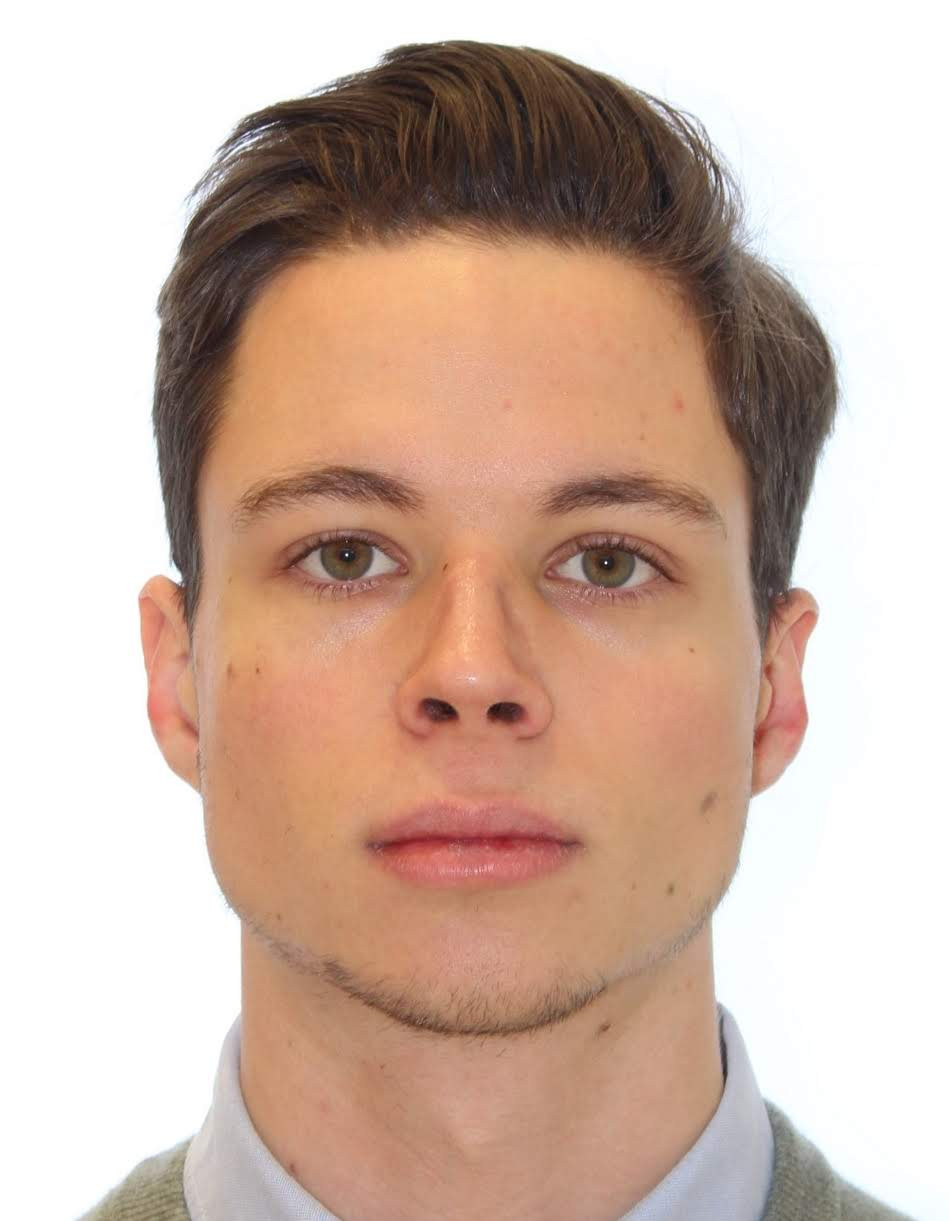
\includegraphics[width=0.5\linewidth]{me}
    % \end{minipage}
    % \vspace{0.5cm}

    %%%%%%%%%%%%%%%%%%%%%%%%%%%%%%%%%%%%%%%%%%%%%%%%%%%%%%%%%%%%%%%%%%%
    % First row
    %%%%%%%%%%%%%%%%%%%%%%%%%%%%%%%%%%%%%%%%%%%%%%%%%%%%%%%%%%%%%%%%%%%
    \raggedright\begin{minipage}[c]{0.69\linewidth}

        %%%%%%%%%%%%%%%%%%%%%%%%%%%%%%%%%%%%%%%%%%%%%%%%%%%%%%%%%%%%%%%%%%%
        % Personal details
        %%%%%%%%%%%%%%%%%%%%%%%%%%%%%%%%%%%%%%%%%%%%%%%%%%%%%%%%%%%%%%%%%%%
        \section{PERSONAL DETAILS}

        \noindent\begin{tabularx}{\linewidth}{ll}
           \textbf{Nationality} & French, Canadian
        \end{tabularx}

        \noindent\begin{tabularx}{\linewidth}{lX}
           \emailsymbol    & \href{mailto:louis.pahlavi@mail.utoronto.ca}{louis.pahlavi@mail.utoronto.ca}\\
           \phonesymbol    & +1 (647) 909-5487 \\
           \mailsymbol     & 106 Wineva Ave, Toronto, ON, M4E 2T2, Canada \\
           \homepagesymbol & \href{https:\\lpahlavi.github.io}{lpahlavi.github.io}
        \end{tabularx}

    \end{minipage}
    \hspace{0.01\linewidth}
    \raggedright\begin{minipage}[c]{0.28\linewidth} 
        \centering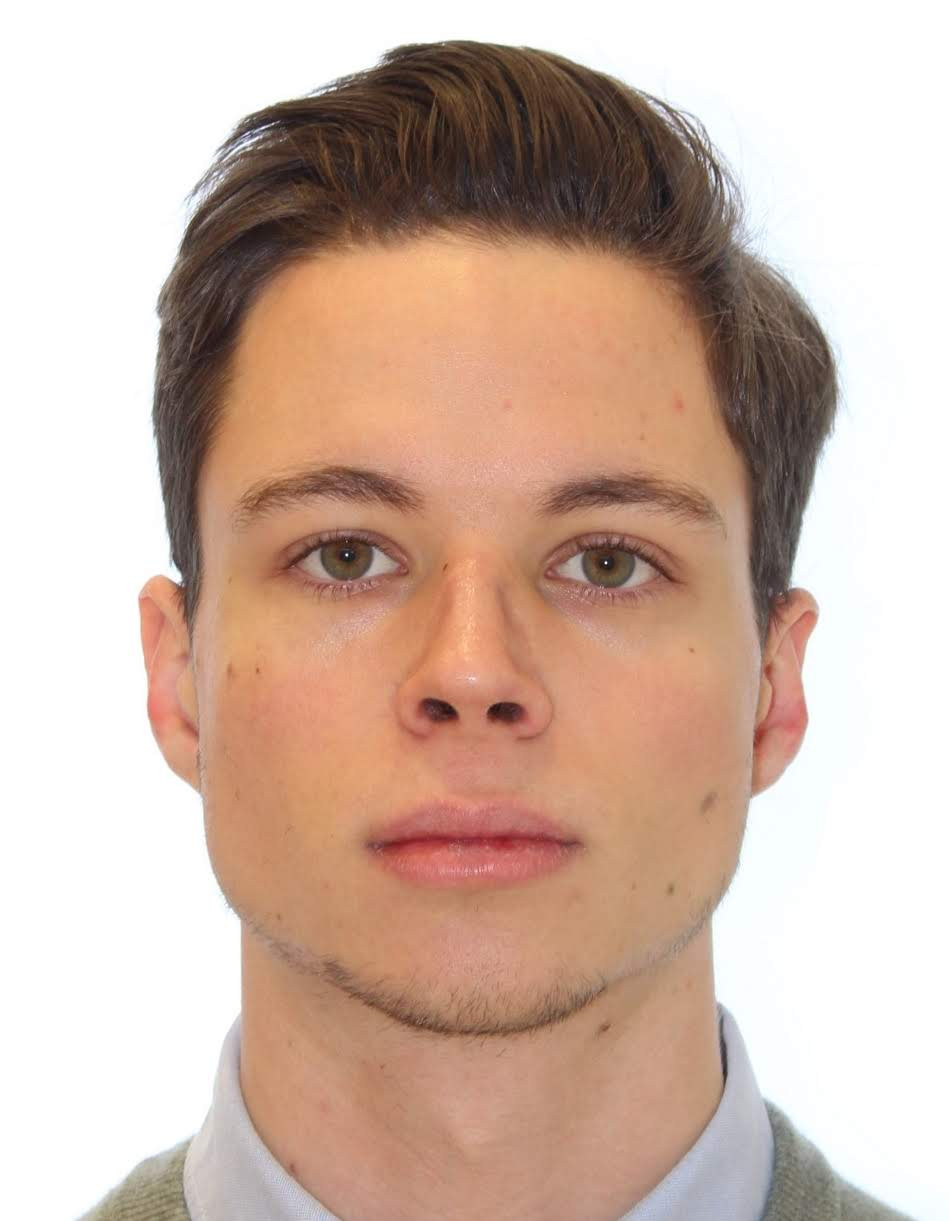
\includegraphics[width=0.65\linewidth]{me}

        % %%%%%%%%%%%%%%%%%%%%%%%%%%%%%%%%%%%%%%%%%%%%%%%%%%%%%%%%%%%%%%%%%%%
        % % Languages
        % %%%%%%%%%%%%%%%%%%%%%%%%%%%%%%%%%%%%%%%%%%%%%%%%%%%%%%%%%%%%%%%%%%%
        % \section{LANGUAGES}

        % \cvskill{English}{5}
        % \cvskill{French}{5}
        % \cvskill{Italian}{4}
        % \cvskill{German}{3}
        % \cvskill{Czech}{1}
    \end{minipage}
    \vspace{0.5cm}

    %%%%%%%%%%%%%%%%%%%%%%%%%%%%%%%%%%%%%%%%%%%%%%%%%%%%%%%%%%%%%%%%%%%
    % Second row
    %%%%%%%%%%%%%%%%%%%%%%%%%%%%%%%%%%%%%%%%%%%%%%%%%%%%%%%%%%%%%%%%%%%
    \raggedright\begin{minipage}[t]{0.69\linewidth} 

        %%%%%%%%%%%%%%%%%%%%%%%%%%%%%%%%%%%%%%%%%%%%%%%%%%%%%%%%%%%%%%%%%%%
        % Technical Skills
        %%%%%%%%%%%%%%%%%%%%%%%%%%%%%%%%%%%%%%%%%%%%%%%%%%%%%%%%%%%%%%%%%%%
        \section{TECHNICAL SKILLS}

        \noindent\begin{tabularx}{\linewidth}{>{\bfseries}lX}
           Build tools     & Makefile, CMake \\
           Version control & Git \\
           Platforms       & Linux, Raspberry Pi, Arduino \\
           Libraries       & Boost, QT, CVX, Tensorflow \\
           Theory          & Control theory and robotics, Networking, Optimization, Algorithms and data structures, Machine learning
        \end{tabularx}
    \end{minipage}
    \hspace{0.01\linewidth}
    \raggedright\begin{minipage}[t]{0.28\linewidth} 
        %%%%%%%%%%%%%%%%%%%%%%%%%%%%%%%%%%%%%%%%%%%%%%%%%%%%%%%%%%%%%%%%%%%
        % Programming languages
        %%%%%%%%%%%%%%%%%%%%%%%%%%%%%%%%%%%%%%%%%%%%%%%%%%%%%%%%%%%%%%%%%%%
        \section{PROGRAMMING LANGUAGES}

        \cvskill{C/C++}{5}
        \cvskill{Python}{5}
        \cvskill{MATLAB}{4}
        \cvskill{Java}{2}

    \end{minipage}

    %%%%%%%%%%%%%%%%%%%%%%%%%%%%%%%%%%%%%%%%%%%%%%%%%%%%%%%%%%%%%%%%%%%
    % Education
    %%%%%%%%%%%%%%%%%%%%%%%%%%%%%%%%%%%%%%%%%%%%%%%%%%%%%%%%%%%%%%%%%%%
    \section{EDUCATION}

    % \datedsubsection{ETH Z{\"u}rich, MSc in Computational Science}{September 2019--February 2021}

    % \workitemsone
    % {Specialization in Financial Engineering}

    \datedsubsection{University of Toronto, BASc in Computer Engineering}{September 2014--April 2019}

    \workitemsfour
    {Minor in Robotics and Mechatronics}
    {Final Project: \textit{Distributed Formation Control of a Swarm of Unicycles}}
    {16 month internship between third and fourth years of studies}
    {Latest term 92.1\% average (ranked 4 out of 173), 3.86/4.00 CGPA}

    %%%%%%%%%%%%%%%%%%%%%%%%%%%%%%%%%%%%%%%%%%%%%%%%%%%%%%%%%%%%%%%%%%%
    % Research and industry experience
    %%%%%%%%%%%%%%%%%%%%%%%%%%%%%%%%%%%%%%%%%%%%%%%%%%%%%%%%%%%%%%%%%%%
    \section{RESEARCH AND INDUSTRY EXPERIENCE}
    
    % Verity Studios
    \position{Systems and Control Engineering Intern}{May 2017--August 2018}{\href{https://veritystudios.com/}{Verity Studios AG}}{Z{\"u}rich, Switzerland}

    \workitemsfour
    {Worked on improving the onboard estimation and control algorithms of swarms of quadcopters implemented in C++.}
    {Evaluated and characterized flight performance and effectiveness of calibration routines using Python and successfully improved drone production pipeline.}
    {Serviced entertainment drone show systems overseas and personally oversaw flight operations for several weeks.}
    {Maintained and improved offboard control and housekeeping applications including Graphical User Interfaces (GUIs).}
    
    % LBB
    \position{Researcher}{May 2016--August 2016}{\href{http://www.lbb.ethz.ch/}{ETH Z{\"u}rich Laboratory for Biosensors and Bioelectronics}}{Z{\"u}rich, Switzerland}
    
    \workitemsthree
    {Developed the control and image processing software for a biosensor measuring protein interactions in fluids.}
    {Created a GUI using QT to control the actuators and interface them with various sensors including a live camera feed and calibration procedures.}
    {Experimented on the growth of networks of living animal neurons.}

    % UTIAS-SFL
    \position{Radio Frequencies Engineer}{June 2015--September 2015}{\href{https://www.utias-sfl.net/}{University of Toronto Institute for Aerospace Studies - Space Flight Laboratories}}{Toronto, Canada}

    \workitemstwo
    {Designed and simulated the early prototypes of a deployable antenna mounted on the NORSAT-2 maritime communications satellite (launched in 2017) in collaboration with the European Space Agency.}
    {Built, tested and tuned antenna prototypes including validation using a Vector Network Analyzer (VNA).}
    
    % UofT EM Lab
    \position{Researcher}{May 2015--June 2015}{\href{http://www.waves.utoronto.ca/prof/svhum/}{University of Toronto Reconfigurable Antenna Laboratory}}{Toronto, Canada}
    
    \workitemsone
    {Created a MATLAB simulation to model a satellite's orbit and predict antenna radiation intensity on the surface of the Earth. Worked on antenna synthesis to find an antenna array for a given desired coverage area.}
    
    %%%%%%%%%%%%%%%%%%%%%%%%%%%%%%%%%%%%%%%%%%%%%%%%%%%%%%%%%%%%%%%%%%%
    % Projects and Teaching
    %%%%%%%%%%%%%%%%%%%%%%%%%%%%%%%%%%%%%%%%%%%%%%%%%%%%%%%%%%%%%%%%%%%
    \section{PROJECTS} % AND TEACHING}
    
    % Capstone
    \position{Capstone Team Lead}{September 2018--April 2019}{\href{https://www.engineering.utoronto.ca/}{University of Toronto Faculty of Engineering}}{Toronto, Canada}

    \workitemsthree
    {Implementing a fully distributed algorithm for the formation control of a swarm of wheeled robots in C++.}
    {Built and tested the communication interfaces between onboard modules and C++ and Python applications.}
    {Developed a Python simulation framework to test and tune the control algorithms. }
    
    % % APS100
    % \position{Teaching Assistant}{September 2016--December 2016}{\href{https://www.engineering.utoronto.ca/}{University of Toronto Faculty of Engineering}}{Toronto, Canada}

    % \workitemsone
    % {Taught APS100 -- 'Orientation to Engineering' to first year Electrical and Computer Engineering students.}
    
    % UTAT SS
    \position{Wireless Communications Lead}{September 2014--June 2016}{\href{https://www.utat.ca/space-systems/}{University of Toronto Aerospace Team (Space Systems)}}{Toronto, Canada}

    \workitemstwo
    {Designed, built and tested the antenna and communication module PCB, on a student-built nano-satellite.}
    {Presented our design at several Product Design Reviews and the Critical Design Review in Vancouver.}

    % % 330 Danforth Tech
    % \position{Ground School Instructor}{September 2014--January 2015}{330 Danforth Tech Royal Canadian Air Cadet Squadron}{Toronto, Canada}
    
    % \workitemsone
    % {Coordinated and taught the pilot ground school course at 330 Danforth Tech Royal Canadian Air Cadet Squadron leading several of my students to earn their pilot wings.}

    %%%%%%%%%%%%%%%%%%%%%%%%%%%%%%%%%%%%%%%%%%%%%%%%%%%%%%%%%%%%%%%%%%%
    % Scholarships and awards
    %%%%%%%%%%%%%%%%%%%%%%%%%%%%%%%%%%%%%%%%%%%%%%%%%%%%%%%%%%%%%%%%%%%
    \section{SCHOLARSHIPS AND AWARDS}
    \begin{itemize}[noitemsep, leftmargin=*]
        \item \textbf{Faculty of Applied Science and Engineering Dean's Honours List} \hfill 2014--Present
        \item \textbf{Gordon R. Slemon Scholarship} -- Awarded for engineering design and academic excellence \hfill 2016
        \item \textbf{University of Toronto International Exchange Bursary} \hfill 2016
        \item \textbf{University of Toronto Centre for International Exchange Award} \hfill 2016
        \item \textbf{Royal Canadian Air Cadet Power Pilot Scholarship} \hfill 2014
        \item \textbf{Royal Canadian Air Cadet Glider Pilot Scholarship} \hfill 2013
    \end{itemize}

\end{document}